\chapter{Walkthrough}\label{ch:walkthrough}
\begin{figure}[h!]
    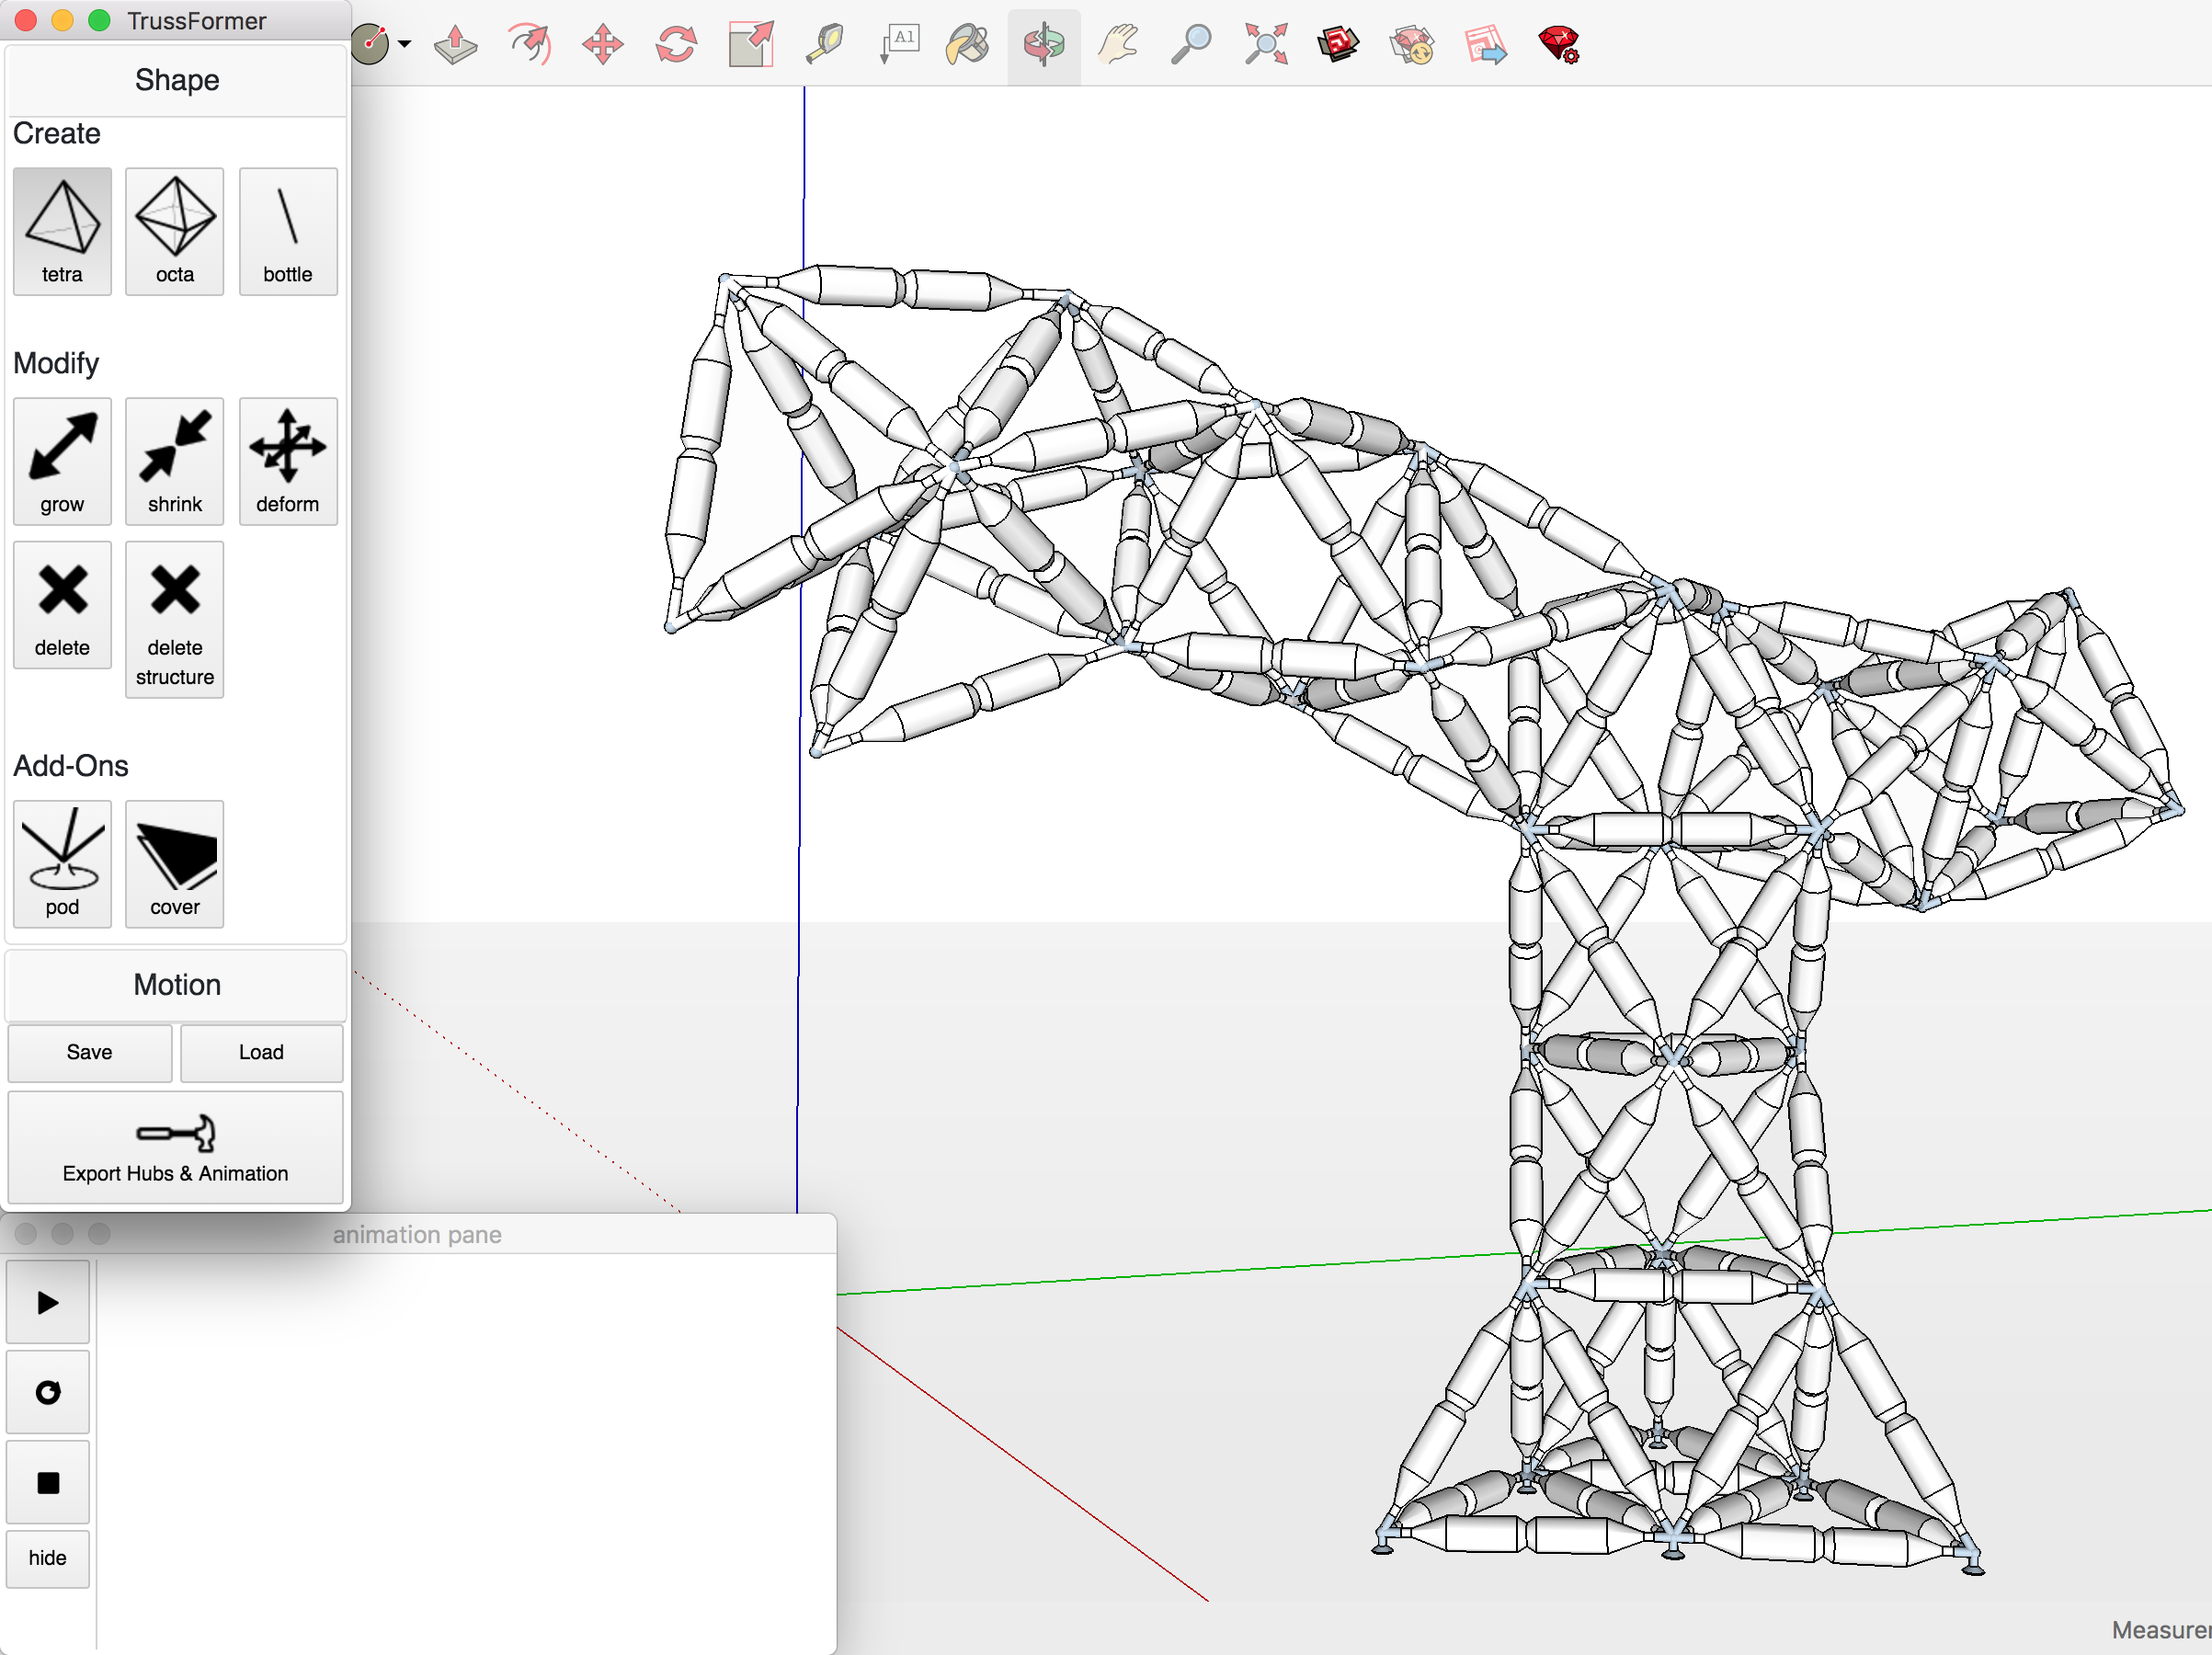
\includegraphics[width=\textwidth]{Walkthrough/dino.png}
    \centering
    \caption{The T-Rex built in TrussFab}
    \label{fig:t_rex}
\end{figure}\improvement{Don't show animation pane...}
This chapter will present the functionalities of the system by showing the process of creating the T-Rex shown in figure \todo{Add image}. This will include all steps from creating the static structure, over introducing animation up to fabricating the final object.

\section{Designing Static Structures}
Users can use predefined and structurally stable primitives to create their objects. These primitives are tetrahedra and octahedra. The structure can be formed as desired by using the grow and shrink tool. These tools elongate or shorten edges, deforming the structure dynamically in such a way that the form stays in tact as much as possible. The deform tool does a similar job, but rather than working on edges, this tool can move nodes.\\
The created Objects can also be saved to a JSON file. This way the user can either save his work for working on it later or create new primitives that can be attached to another object.
\begin{figure}
  \centering
  \begin{minipage}{.5\textwidth}
    \centering
    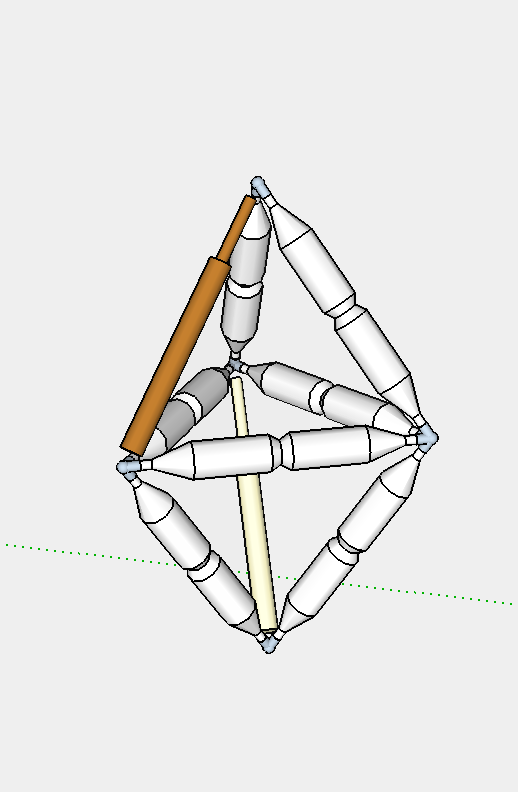
\includegraphics[width=.9\linewidth]{Walkthrough/leg_asset.png}
    \captionof{figure}{An exported leg asset...}
    \label{fig:leg_asset}
  \end{minipage}%
  \begin{minipage}{.5\textwidth}
    \centering
    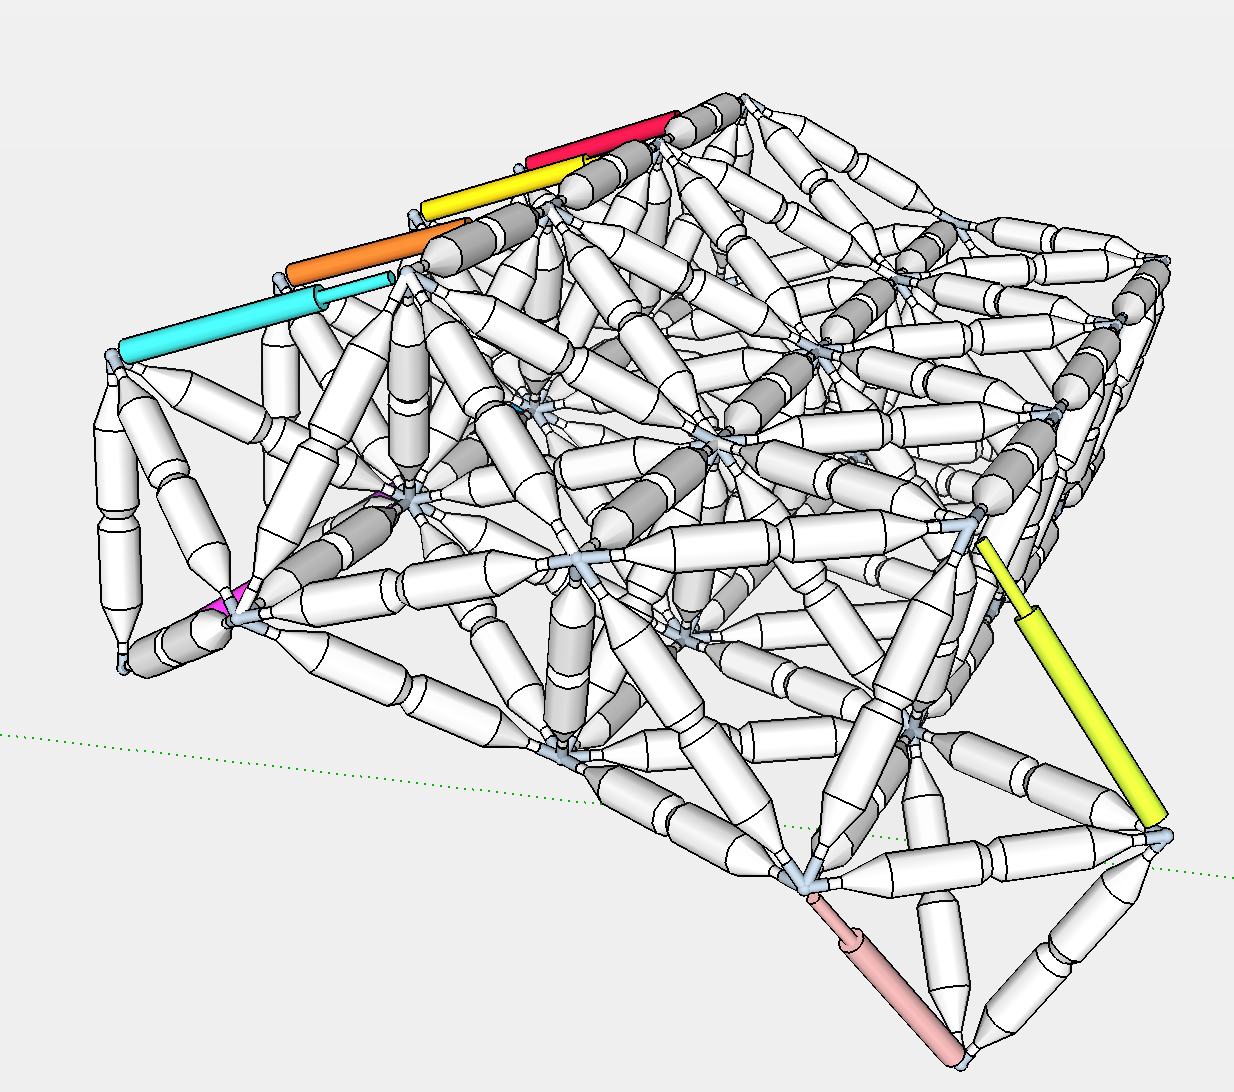
\includegraphics[width=.9\linewidth]{Walkthrough/spider_using_leg_asset.png}
    \captionof{figure}{... which can be used to quickly build the spider}
    \label{fig:spider_in_progress}
  \end{minipage}
\end{figure}

\section{Adding Movement to the Structures}
Movement is added to the structure by placing special physics links. These links act like linear actuators - struts that can extend and retract in a straight line. There are multiple methods for placing these actuators, ranging from a fully-automated way to manual placement.
\begin{figure}
  \centering
  \begin{minipage}{.5\textwidth}
    \centering
    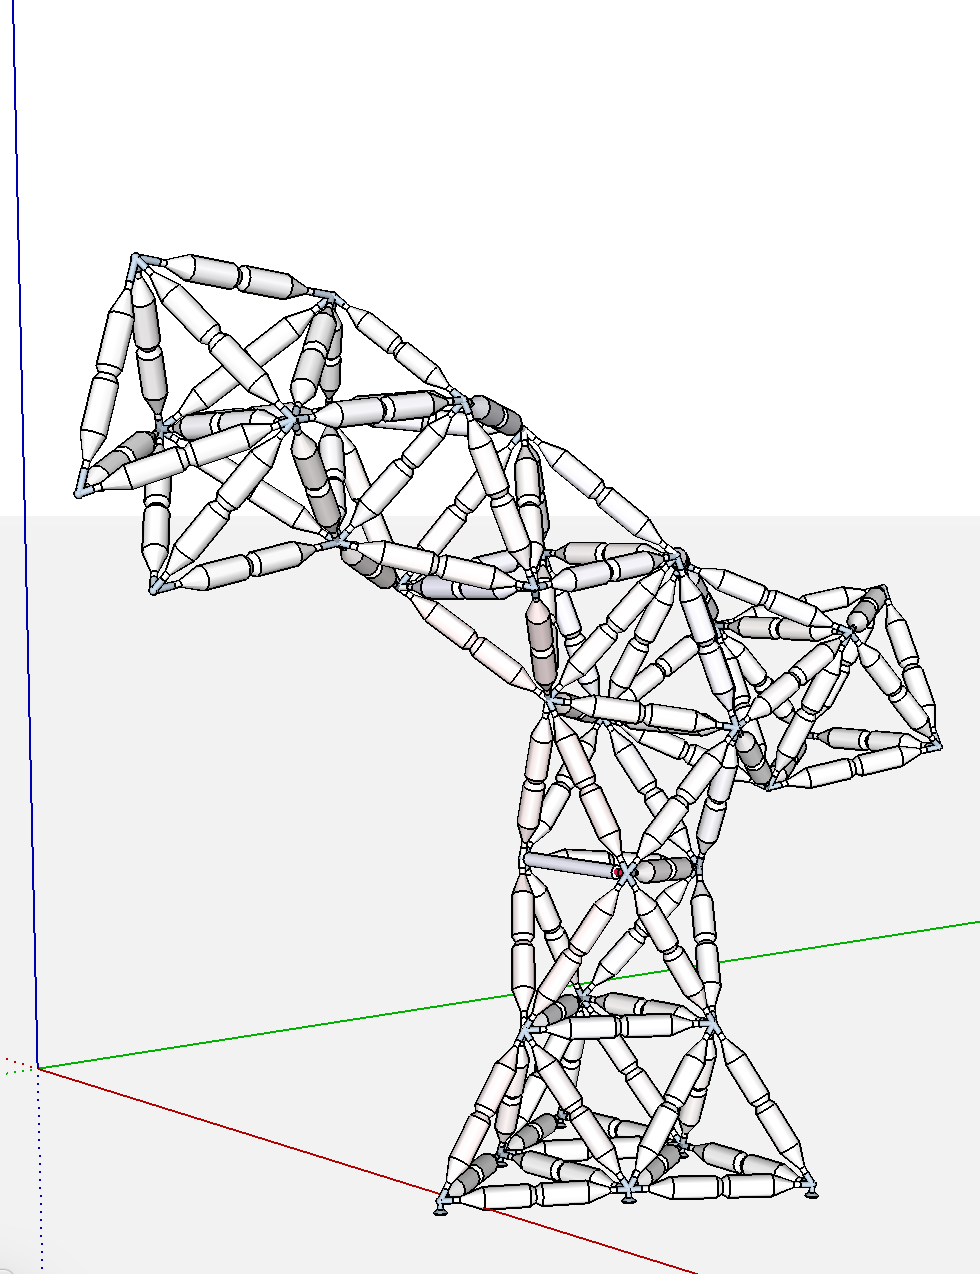
\includegraphics[width=.9\linewidth]{Walkthrough/crane_up.png}
    \captionof{figure}{An exported leg asset...}
    \label{fig:dino_up}
  \end{minipage}%
  \begin{minipage}{.5\textwidth}
    \centering
    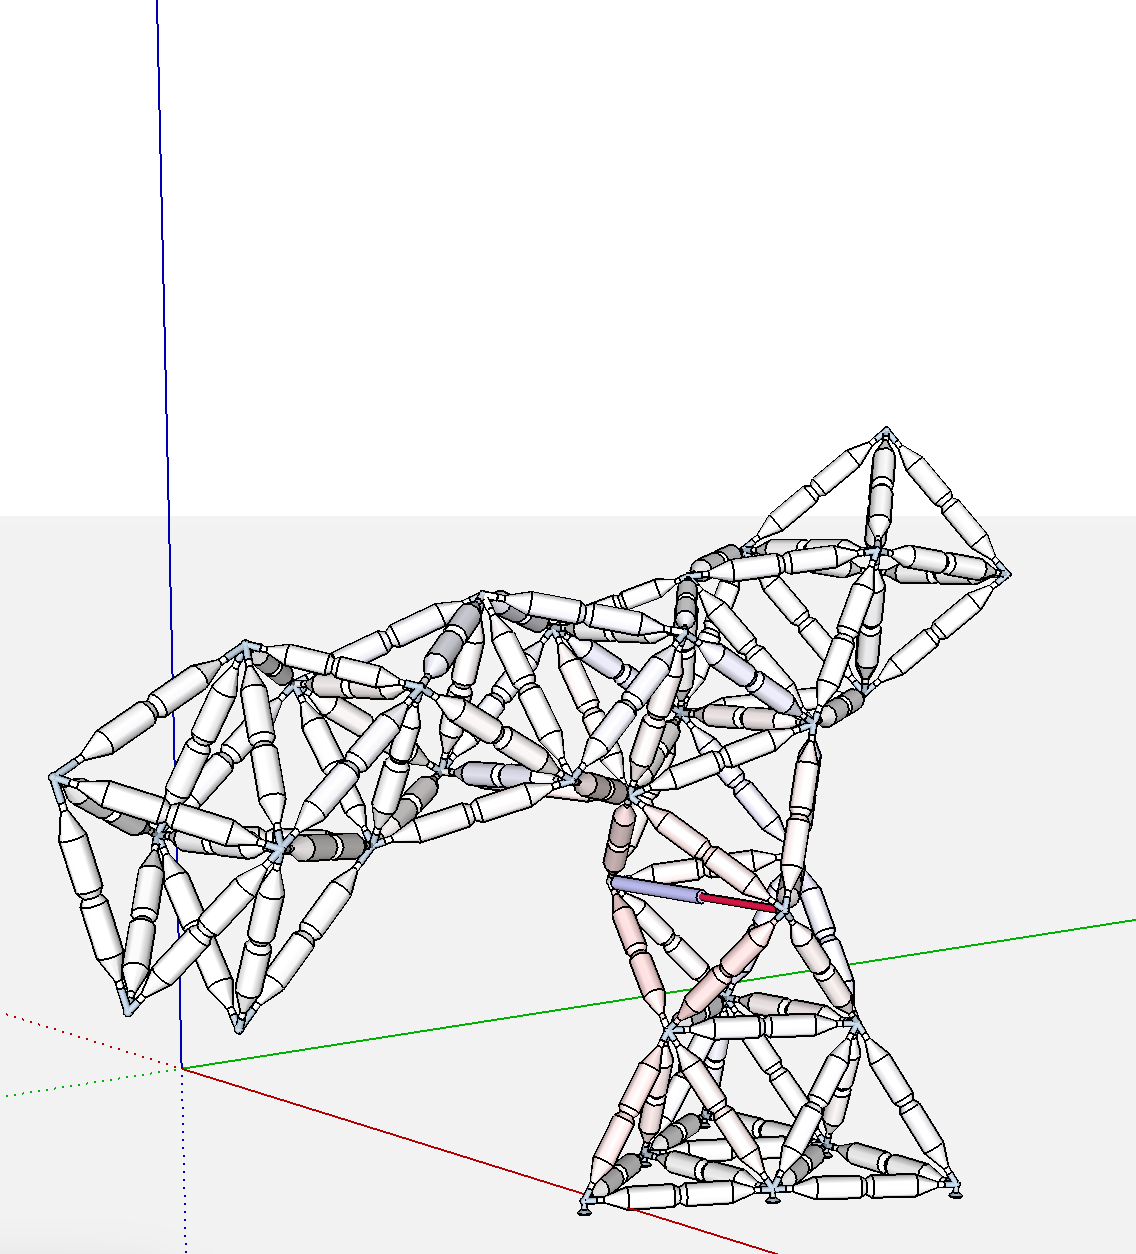
\includegraphics[width=.9\linewidth]{Walkthrough/crane_down.png}
    \captionof{figure}{... which can be used to quickly build the spider}
    \label{fig:dino_down}
  \end{minipage}
\end{figure}\todo{Caption!}
The automated way works by demonstrating a desired movement. The user selects the \textit{Demonstrate Movement Tool}, clicks a node that should experience a certain movement and drags a line to the desired end position. TrussFab will then search for an actuator that brings the node closest to the desired position and turns the resulting edge into an actuator. The tool runs through all edges of the structure, replacing one after another with an actuator and simulates the resulting movement in the background. The actuator that solves the problem the best will be created.\\
Another way to add movement is to use predefined dynamic assets. It can be difficult for a user to fully grasp how an actuator will move the whole object. That's why we encapsulated often-used atomic sub-assemblies into quick-access tools. These assets connect to the rest of the structure through a dedicated triangle surface. Because the motion is localized in this asset, the result in the bigger structure is easier understandable.\\
The manual actuator placement requires the most knowledge about the resulting motion. It is, however, the most flexible way to create movement. The user can choose the actuator tool to turn every edge into or connect two nodes with an actuator. This can be done by clicking on the desired edge or the nodes. Transforming an existing edge is usually the desired use case, as the introduction of more edges (by connecting two previously unconnected nodes) tends to make the truss more stable and can prevent motion altogether. Turning an edge into an actuator essentially removes this edge and adds a degree of freedom.\\
The user can actuate these links in two different ways. The \textit{animation window} provides a slider for manual movement, as well as an animation pane which allows placing keyframes and playback modes: single and looping. All actuators have an actuators group assigned to them. Per default, an actuator is placed in its own, empty group. Using the actuator tool, already used for placing actuators, this group can be changed, which is indicated by the actuator changing its color.\\
Control elements of the animation window always work on the whole group. The color of the animation line indicates which group will be actuated by either the slider or the keyframes.
\begin{figure}[h!]
    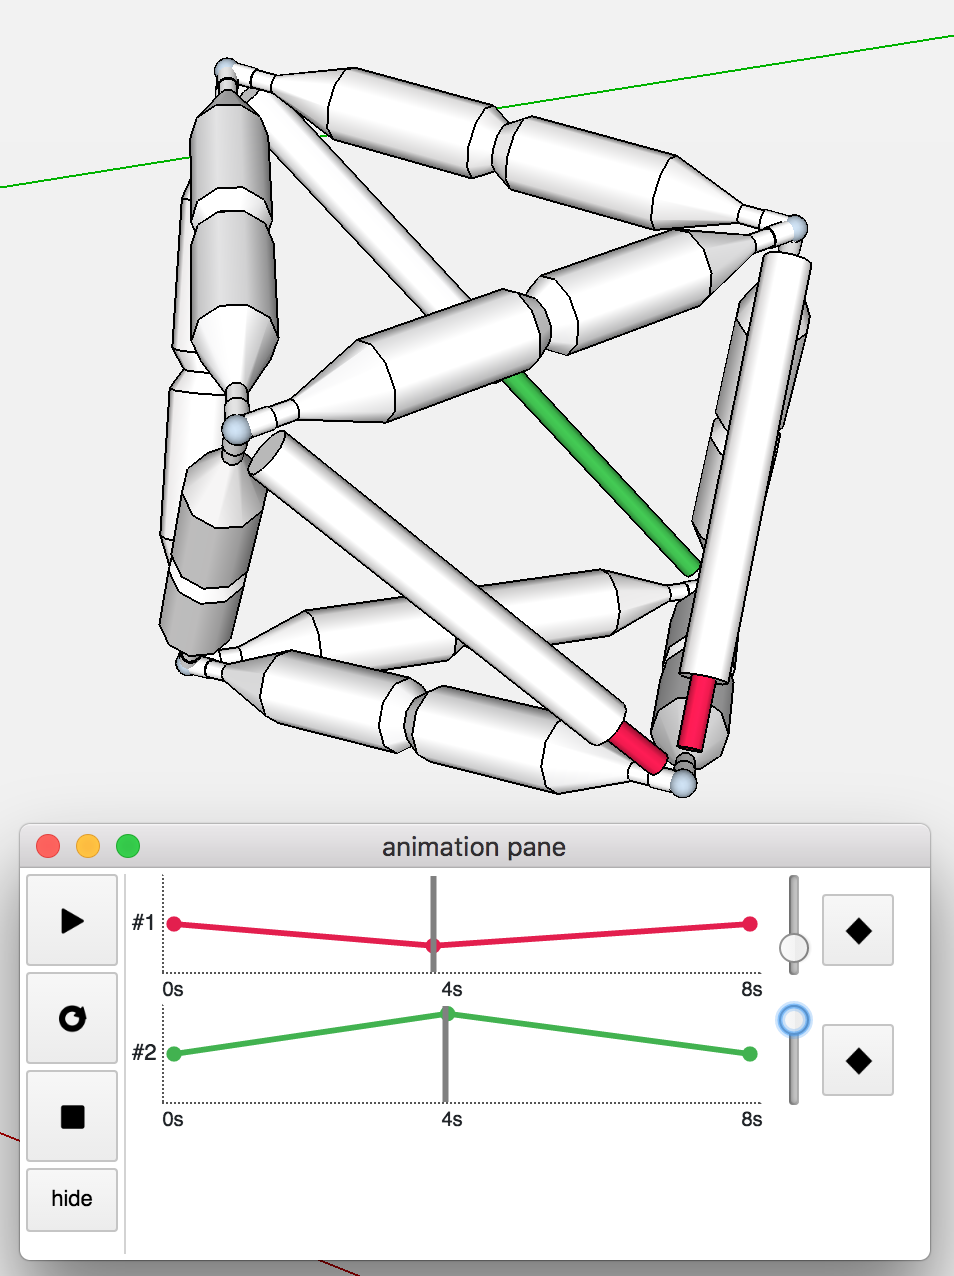
\includegraphics[width=.5\textwidth]{Walkthrough/animation_pane.png}
    \centering
    \caption{The animation pane showing two actuators group, the red one contains two actuators}
    \label{fig:animation_pane}
\end{figure}
To add a keyframe to the animation pane, first the slider has to be moved to the desired position. The object will start to move according to the sliders position - if the slider is at the top, the actuator will be fully extended and vice versa. That way, the user can visualize the extend of the movement. If the user is satisfied, the indicator line can be moved to the desired position in the timeline and the diamond button is pressed to add this point to the animation.

\subsection{Force Analysis}
If the structure fulfills the desired motion, the user will want to check if the forces created during executing it will not exceed the breaking force of the object. A lot of factors play a role in the formation of the forces. These range from weight forces over lever forces to inertial forces. TrussFab aids the user to detect weak points and force peaks during a motion in different ways.\\
TrussFab's tools provide the possibility to constantly monitor the forces that occur during interactive movement of the structure. In simulation mode, all edges will be colored red or blue in increasing intensity the higher the force on them is. Red indicates compression force, while blue means tension force. A completely white color indicates a force of 0 N. These tension forces are automatically calculated by the built-in physics engine.\\
The weight of each node, which plays a big role in the force distribution, is calculated based on the number of edges connected to it and whether it is a hinge or a hub. If the user decides that certain nodes will have more load, these can be fitted with additional weight using the \textit{Add Weight Tool}.\\
On top of the coloring of edges, the user can also use a sensor tool. This tool can be used on a single edge and observes this one more closely. The force data on an edge with a sensor will be recorded and visualized over time in a chart. This tool also works on nodes. Rather than recording the force, if the sensor tool is used on nodes, speed and acceleration data will be visualized. The result can be seen in figure \ref{fig:sensor}.\\
\begin{figure}[h!]
    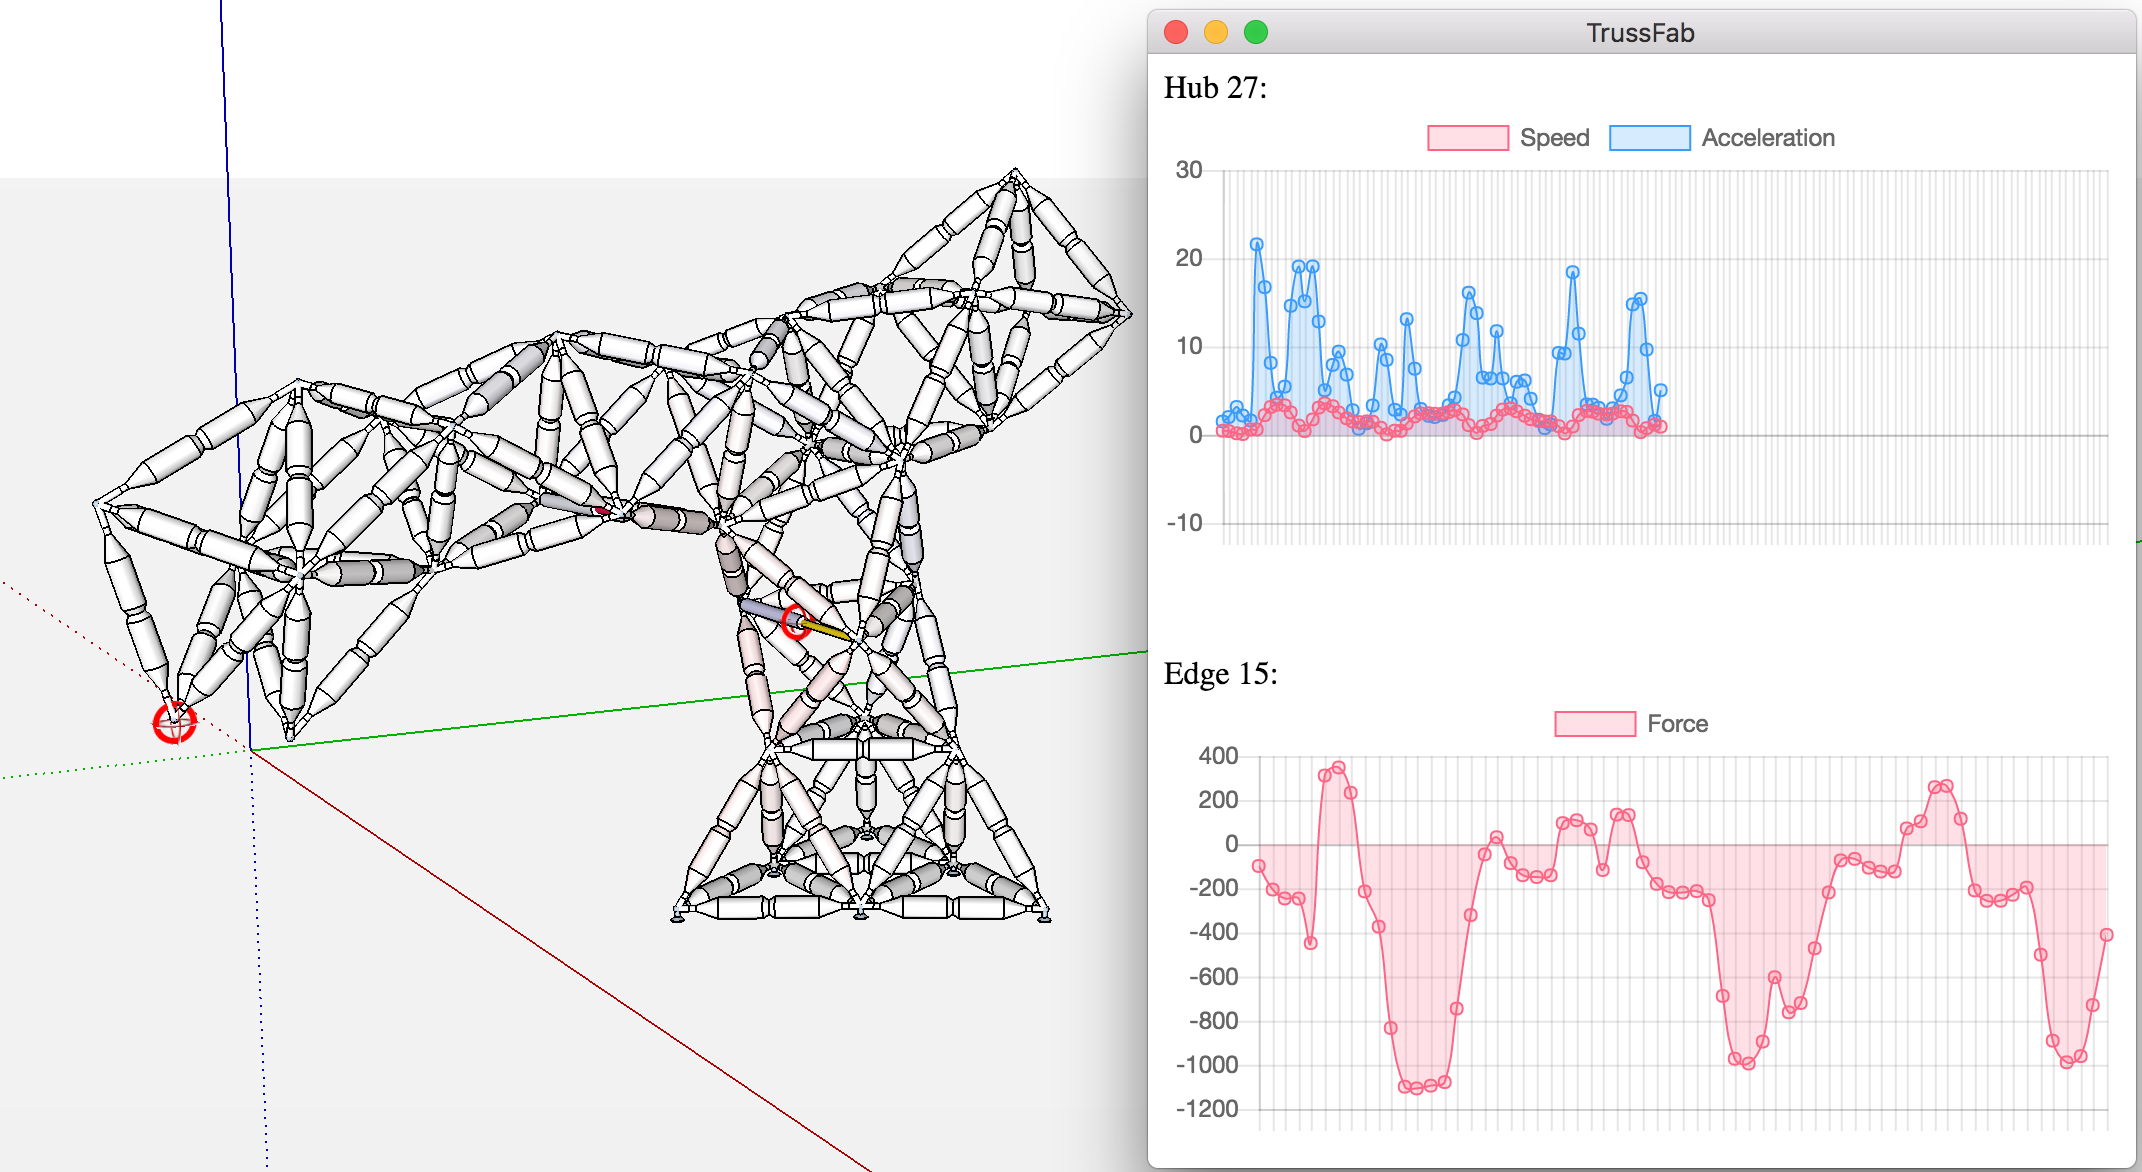
\includegraphics[width=\textwidth]{Walkthrough/sensor.png}
    \centering
    \caption{A sensor measures the force on the central actuator, and speed and acceleration on a node at the ``nose'' of the dino}
    \label{fig:sensor}
\end{figure}
Using these tools, the user can detect unwanted movements, like wobbling during change of poses, overly stressful actuations and even foresee breaking points.\\
If the movement of an animation exceeds the breaking force of the simulation, TrussFab has means of helping the user to find a movement curve that puts less stress on the structure. If TrussFab detects that the structure broke, a popup window will appear asking the user to fix the animation. Two possibilities are available: fixing the animation by a) reducing the speed or b) reducing the motion. If option a) is chosen, TrussFab will elongate the animation sequence for all piston groups. This results in a slower movement and less force on the structure. Option b) will keep the length of the animation, but move the keyframes closer to the center line. The amplitude of the motion will be decreased this way.\\
Both versions will reduce the acceleration of the structure. The force formula $F = m * a$ shows, that the force increases proportionally with the acceleration, as the mass is constant in the structure. Reducing acceleration also reduces the force.
\begin{figure}[h!]
    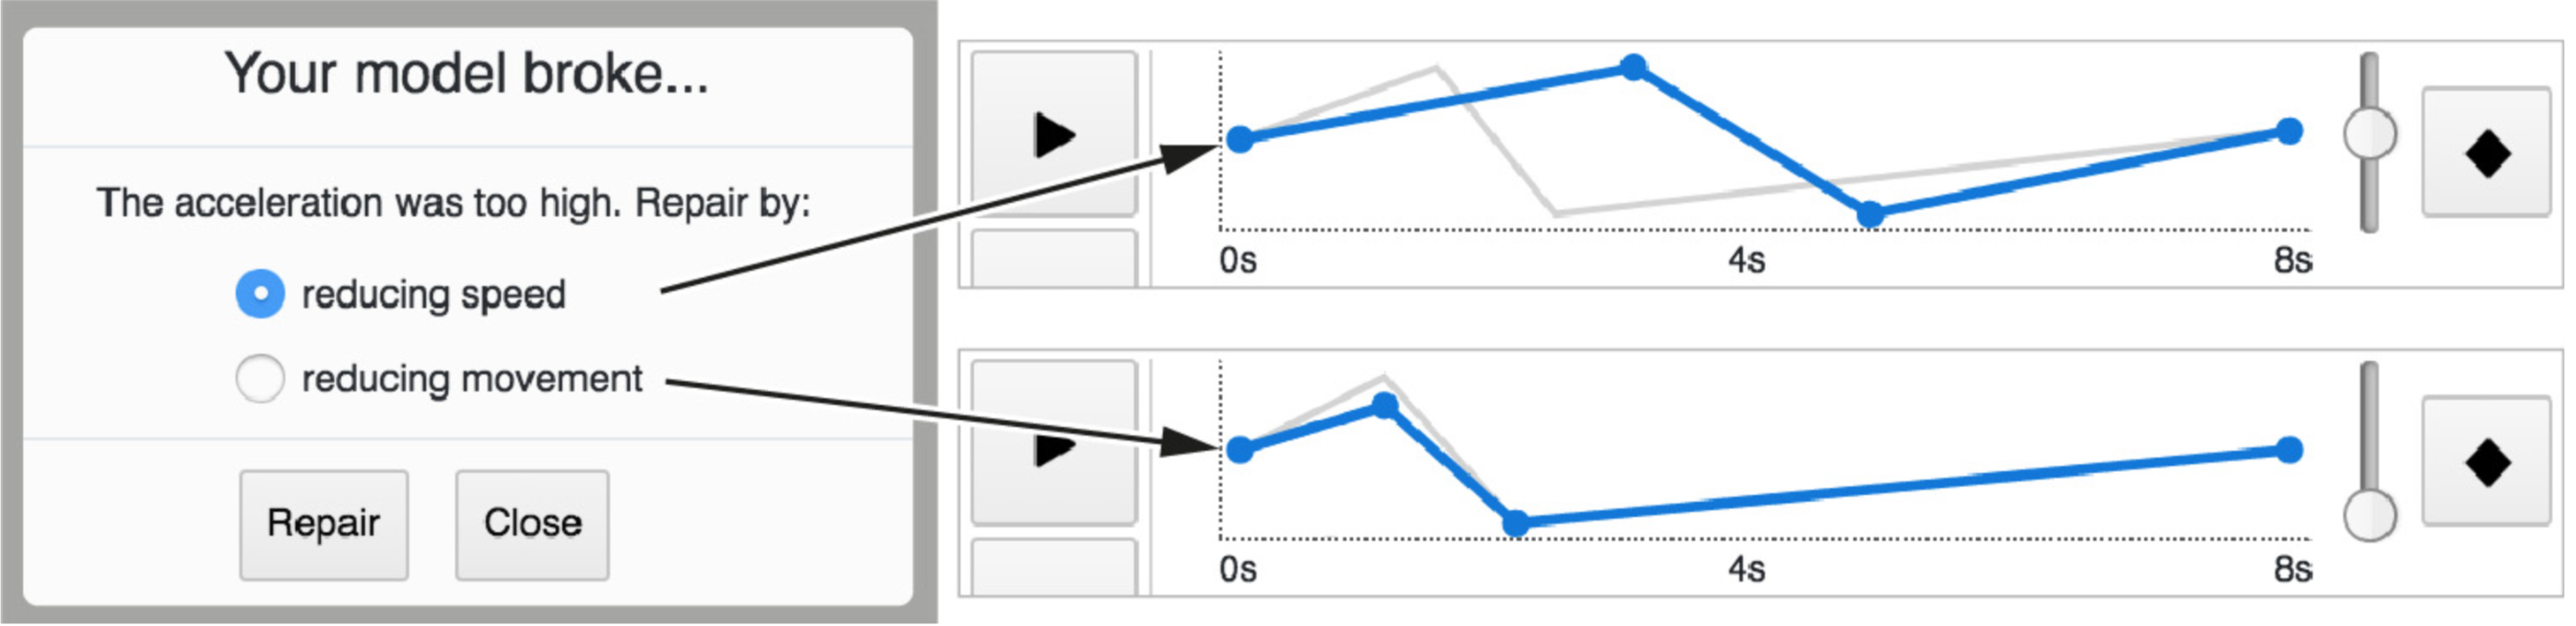
\includegraphics[width=\textwidth]{Walkthrough/fix_breaking.png}
    \centering
    \caption{adsf}
    \label{fig:fix_breaking}
\end{figure}

\section{Controlling the Structure}
Pneumatic actuators themselves do not have any knowledge about their position and extent. Their actuation underlies so-called open-loop control, meaning that the actuator can not react to changing external influences.
- closed-loop control -> more sophisticated and complex movements possible\\

\subsection{PID Control}
- short intro: how does PID work?\\
- how do we use it?\\
- i.e. position control of actuators\\
- forward reference to section 4 (setup of length measurement)\\

\section{Building the Final Object}
After the object was sufficiently tested in the editor, it is time to print the connectors and assemble the final object. To do this, TrussFab will calculate which connections will need to move and which can be static in the printed object. It also takes into account constraints, such as the minimum distance from a bottle neck to the center of a hinge, which might otherwise restrict movement. This process will be explained in detail in Section \ref{sec:hinge_placement_impl}. This information is used to create OpenSCAD files - a modeling language which we use to modify templates of hubs and hinges.

\subsection{OpenSCAD}
At first, our abstract description of the object has to be converted into a physical representation. In order to achieve this, we used a modeling language called \textit{OpenSCAD}. The \textit{Export Hubs and Hinges} button will automatically morph the structure into a statically sound object, i.e. it will elongate and shorten edges so, that the ideal amount of movement is possible. \improvement{This needs to be more detailed for sure!!}\\
The resulting arrangement of nodes and edges will be transferred to OpenSCAD. OpenSCAD enables us to create 3D structures programmatically. We use it to create 3-dimensional primitives, such as spheres, cubes or cylinders, and to apply set operations, like \textit{difference} or \textit{union} on them.\\
OpenSCAD provides an editor which can be used to prototype a model. This editor, including some example operations can be seen in Figure \ref{fig:openscad_overview}. We used this editor to create the template functions used for creating the final hinge and hub models. This will be explained in more detail in \ref{sec:openscad_impl}.
\begin{figure}[h!]
    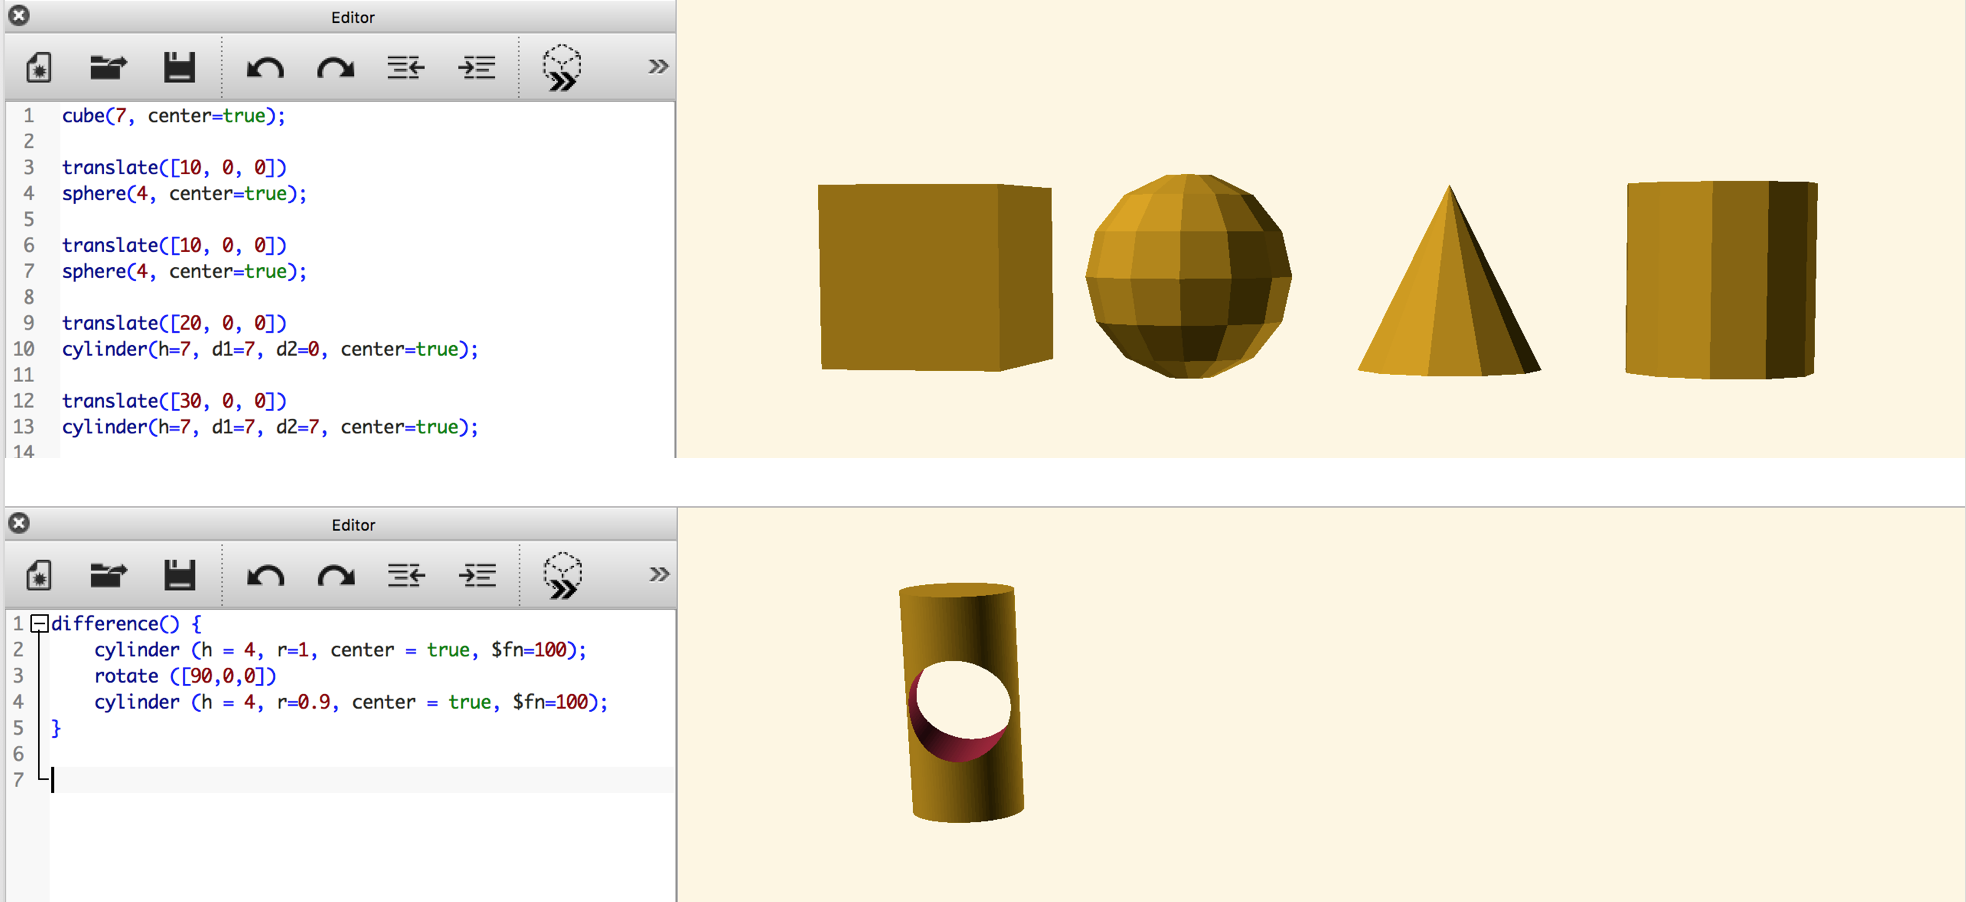
\includegraphics[width=\textwidth]{Walkthrough/openscad_overview.png}
    \centering
    \caption{Overview of the OpenSCAD editor}
    \label{fig:openscad_overview}
\end{figure}

\subsection{Printing the Parts}
Each OpenSCAD file represents a single part in the structure. These files can easily be converted to \textit{.stl} files, which are typically used for 3D printing. These files have to be imported into any 3D printing software, arranged efficiently and sent to a 3D printer. Printing of one hinge part using an UltiMaker 3 printer takes about 20 minutes.\unsure{evaluate!?}

\subsection{Assembling the Structure}
The resulting hubs and hinges contain an ID system for easy assembly. Each part of a node has the node ID printed on. That way it is easy to find out which hinge-parts belong together. Additionally, each edge elongation \info{Verlängerung einer Edge, also quasi die Elongation. FIND A BETTER NAME!} contains the id of the connected edge. A compound elongation, which is the usual case for a hinge, is therefore assembled by finding two parts with the same node and edge ID. For static hubs, this concept is similar, but of course these do not have to be assembled.\\
Two connectors with different node IDs but the same edge IDs will be connected by a link.
\begin{figure}[h!]
    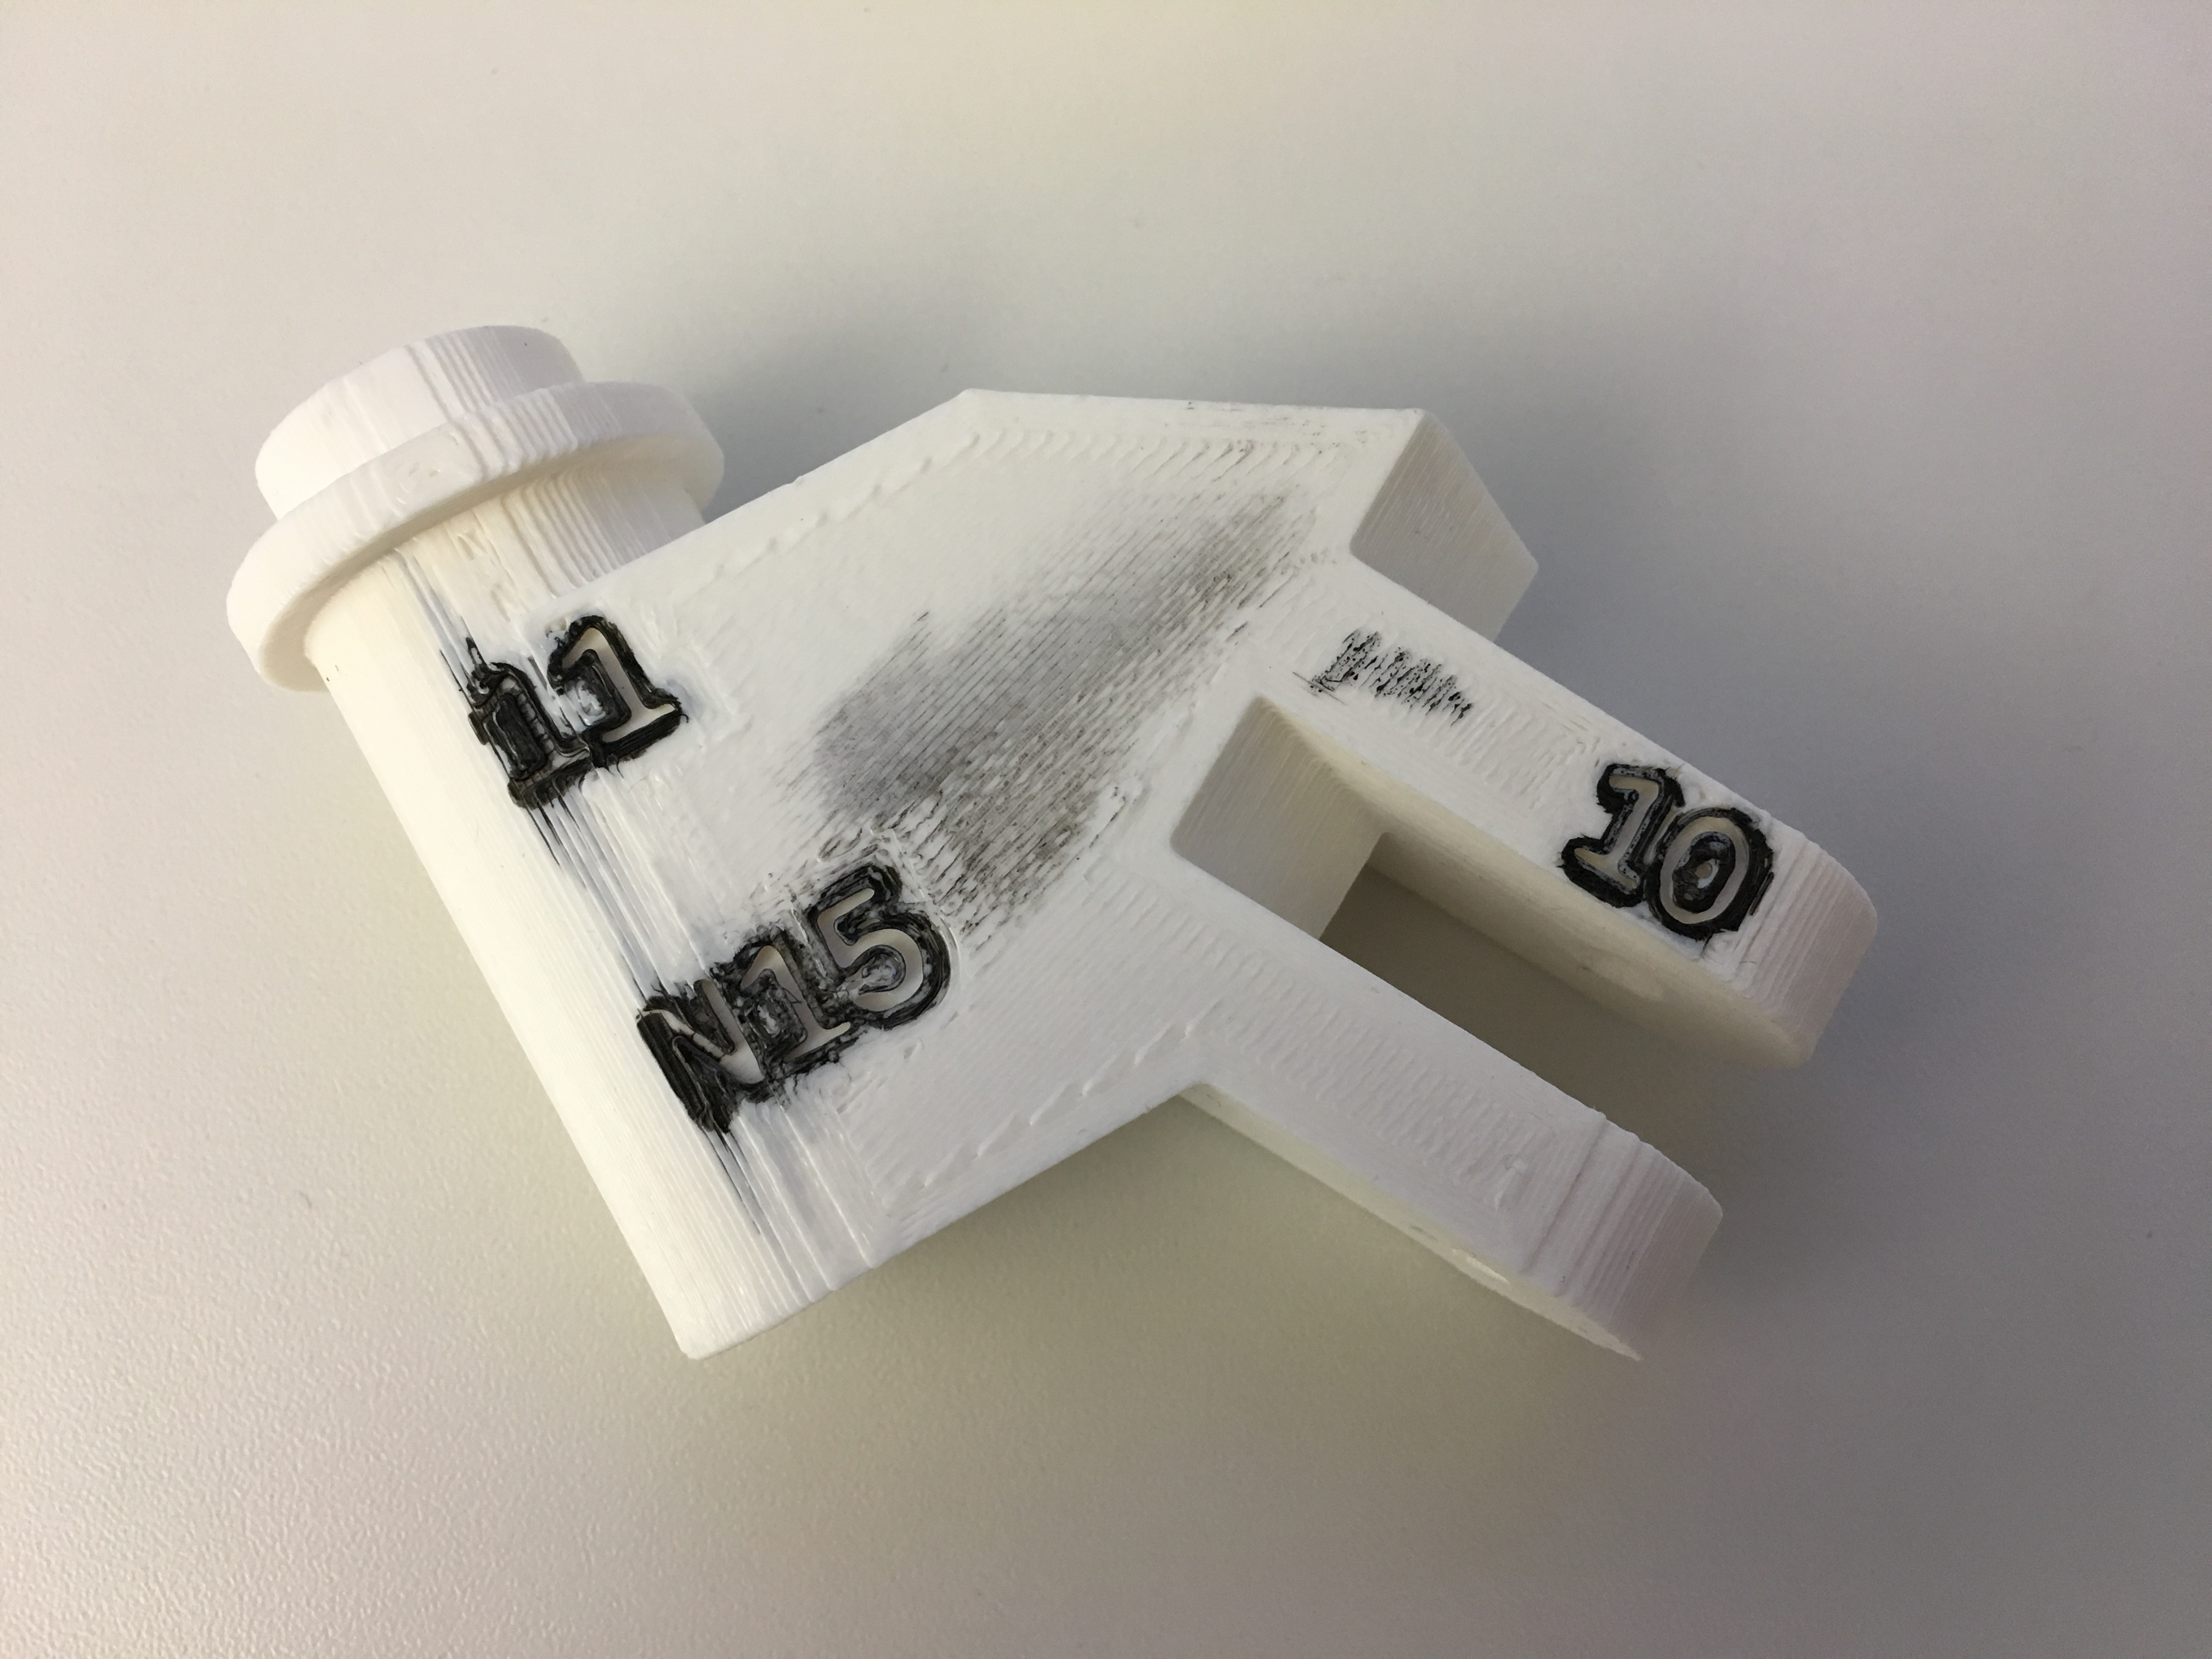
\includegraphics[width=\textwidth]{Walkthrough/hinge.JPG}
    \centering
    \caption{A hinge}
    \label{fig:hinge}
\end{figure}
